\chapter{Installation instruction}
\section{Windows}
\begin{enumerate}
    \item Install Docker for Windows using instructions from: \newline
    https://docs.docker.com/docker-for-windows/install/
    \item Enable hyper-v using instructions from: \newline
    https://docs.docker.com/docker-for-windows/install/
    \item Restart the computer
    \item Click Docker icon in tray and enable option "Switch to Linux Containers..." \newline
        \begin{minipage}{\linewidth}
            \centering
        	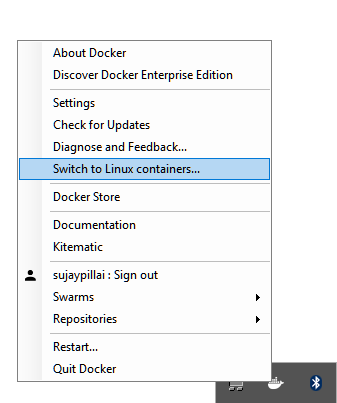
\includegraphics[width=0.4\linewidth]{instructions/systemtray.png}
        \end{minipage}
    \item Optional - open docker settings by clicking settings option and  in adavanced settings adjust how much resources can docker containers use
        \begin{minipage}{\linewidth}
            \centering
        	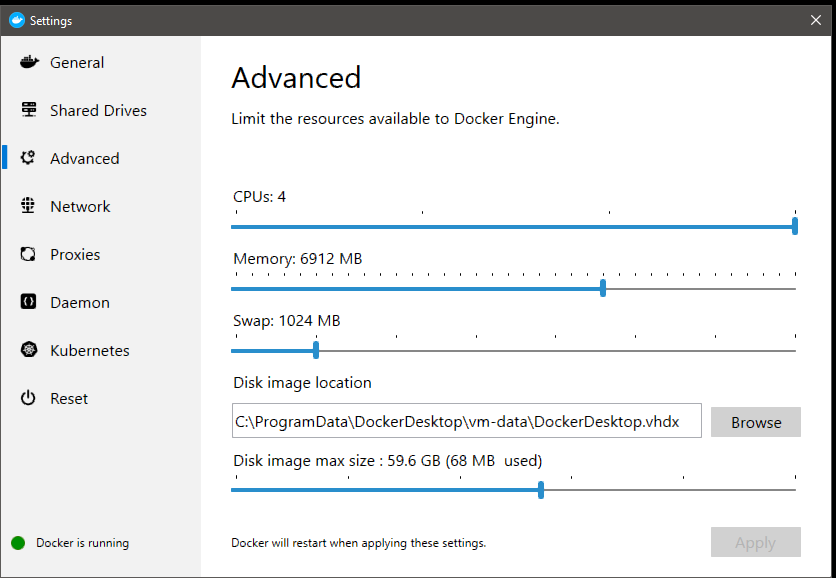
\includegraphics[width=0.4\linewidth]{instructions/res.PNG}
        \end{minipage}
    \item Clone or download repository from: \newline
     https://github.com/JakubSokolowski/simbad-monorepo
    \item Open powershell by pressing windows+R, typing "powershell" and pressing enter.
    \item From inside of powershell change directory to directory when the cloned repository is. The easiest way to do that is to find folder containing repository in Windows Explorer, type "cd " in powershell and drag and drop this folder onto powershell window. The command in powershell should now look like "cd C:\textbackslash Users \textbackslash Alice \textbackslash simbad\-monorepo". Press enter to execute it.
    \item While in cloned folder, enter command docker-compose -f docker/prod-docker-compose.yml up. This will start the download process - this operation may take around 15 mins depending on the internet connection and will download around 4GB of data. \newline
        \begin{minipage}{\linewidth}
            \centering
        	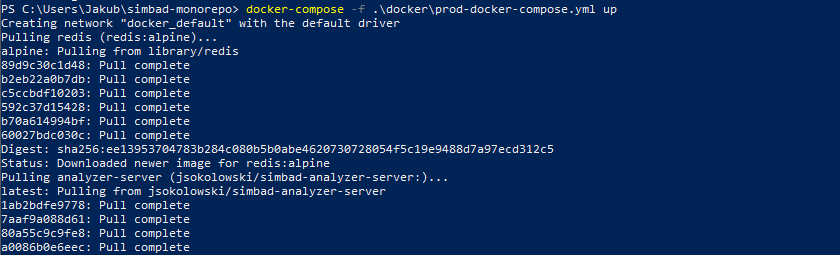
\includegraphics[width=0.9\linewidth]{instructions/docker2.PNG}
        \end{minipage}
    \item Docker will prompt you to enter password for, to grant access to host filesystem. Enter user password for each such prompt. \newline
    \begin{minipage}{\linewidth}
        \centering
        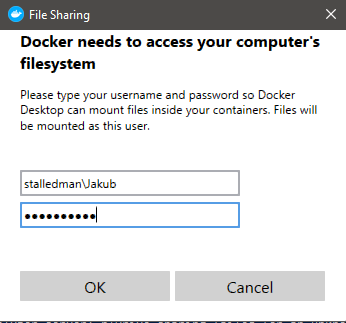
\includegraphics[width=0.5\linewidth]{instructions/docker3.PNG}
    \end{minipage}
    \item After command finishes executing, go to \textit{http://localhost:8080/\#/examples/simulation-pipeline } in browser.
    \item To stop, press ctrl+c in powershell
\end{enumerate}
\section{Linux}
\begin{enumerate}
    \item Install Docker using instructions from: \newline
    \textit{https://docs.docker.com/install/}
    \item Install Docker Compose using official instructions from: \newline
    \textit{https://docs.docker.com/compose/install/}
    \item Clone or download repository from: \newline
     https://github.com/JakubSokolowski/simbad-monorepo
    \item Open the terminal in the root folder of cloned repository
    \item Enter command docker-compose -f docker/prod-docker-compose.yml up. This will start the download process - this operation may take around 15 mins depending on the internet connection and will download around 4GB of data.
    \item Go to \textit{http://localhost:8080/\#/examples/simulation-pipeline } in browser
    \item To stop, press ctrl+c in terminal
\end{enumerate}